\chapter{Echo-aware Applications of \dEchorate{}}\label{ch:dechorateapp}
\openepigraph{Echoes of the same old psalm\\
Sing with me\\
In unity\\
Join in with me\\}{Leprous, \textit{Mirage}}

\vspace{-2.5em}
\newthought{Synopsis} \marginpar{%
\footnotesize
\textbf{Keywords:} Early reflection, Speech Enhancement, Beamforming, Room Geometry Estimation, Reflector Localization.
\\\textbf{Resources:}
\begin{itemize}
    \item \href{www.github.com/Chutlhu/dEchorate}{\library{dEchorate}\ExternalLink}
    \item \href{www.github.com/Chutlhu/Risotto}{\library{Risotto}\ExternalLink}
    \item \href{www.github.com/Chutlhu/Brioche}{\library{Brioche}\ExternalLink}
\end{itemize}
} \synopsisChDecharateApp

\mynewline
This chapter is the continuation of the work presented in~\cref{ch:dechorate}.
Therefore, it is the results of the collaboration with prof. Sharon Gannot and ing. Pinchas Tandeitnik at the Bar'Ilan University, Israel.
The algorithms presented here are straightforward extensions of the one available in the literature.
Nevertheless, they are presented according to the thesis notation.
In addition, they are  gathered and implemented in the following Python library available online:
\library{dEchorate} related to the \ac{DECHORATE} dataset, \library{Risotto} for \acs{RIR} estimation and \library{Brioche} for echo-aware beamforming.

\section{Echo-aware Spatial filtering}\label{sec:dechorateapp:se}
In the previous chapters, we showed how to integrate echoes for sound source separation (\cref{ch:separake}) and sound source localization (\cref{ch:mirage}).
In this section, we investigate this in the context of spatial filtering.
To this end, we compare two types of spatial filters: echo-agnostic and echo-aware beamformers.
In order to study their empirical potential, we will evaluate their performances on both synthetic and measured data, as available in the \dEchorate{} dataset (\cref{ch:dechorate}).
For all the methods presented in this part of the thesis, we assume that echoes are known.
To this end, we used the annotations that come with the considered dataset.

\subsection{Literature review}
The following paragraphs provide a broad overview of existing beamforming methods, with a specific focus on how they handle echoes.
Spatial filtering methods exist in many forms, one of the most popular of which being \textit{beamforming}.

% In light of the echo-aware processing, the literature of beamforming-based spatial filtering can be dichotomized in the following two classes: echo-agnostic and echo-aware approaches.
\newthought{Echo-agnostic beamformers} do not need any echo-estimation step:
they either ignore their contributions, such as the direct-path beamformers~\citeonly{VanTrees2004Optimum}, or they consider coupling filters between pairs of microphones, using so-called \ReIRdef/~\citeonly{gannot2001signal}.
In their vanilla form, neither approaches compute the full acoustic channels explicitly.
In case of direct-path \DStxtdef/ beamformers, only the \DOA/ of the target source is used to build the so called (relative) steering vector.
Then, in order to cope with distortions due to reverberation, external noise or interfering speakers, the statistical description of such forms of noise can be included in extended beamformer design, such as the \MVDRtxt/ beamformer~\citeonly{VanTrees2004Optimum}.
\\The \ReIRs/ (and their frequency counterparts, \ReTFs/) have been introduced with the explicit purpose of avoiding the computation of the acoustic channel related to each microphone~\citeonly{gannot2001signal}.
\ReIRs/-based beamformers instead of returning the dry source signal, return the reverberant source spatial image as it is recorded at a reference microphone.
Compared to the difficult task of estimating the acoustic channels and of relying on bad channel estimates, this is typically sufficient for achieving good enhancement performances in many practical scenarios.\sidenote{
    Note that, as opposed to channel estimation, estimating the \ReTF/ is a non-blind problem (See~\cref{sec:processing:rirmodels})}
Since then, \ReIRs/ have been incorporated in powerful beamforming algorithms, used for both dereverberation and noise reduction (\eg/ \citeonly{schwartz2014multi, kodrasi2017evd}).

\newthought{Echo-aware beamformers} explicitly model multipath sound propagation instead.
They can be seen as \textit{rake receivers}, borrowing the idea from telecommunication where an antenna \textit{rakes} (\textit{i.e.} combines) coherent signals arriving from different propagation paths.
In particular, they consider ``extended'' steering vectors, whose formulation uses known echo delays and attenuations~\citeonly{flanagan1993spatially,jan1995matched}.
The underlying motivation is two-fold:
on the one hand, they better describe the acoustic propagation of the source signal; on the other hand, the early echoes' energy is included in the estimated signal and not considered noise to be removed.
Later, this approach has been extended to enhance desired signals in the context of the \textit{cocktail party problem} in~\citeonly{Dockmanic2015raking} and for noise and reverberation reduction~\citeonly{peled2013linearly, Javed2016spherical, Kowalczyk2019raking}.
In particular, the work~\citeonly{peled2013linearly} estimates early echoes in the spherical harmonic domain and uses their \DOAs/ to build \ReIR/.
However, this approach is not generalizable to all microphone array configurations as it requires the deployment of (3D) spherical arrays.
Alternatively, the authors of~\citeonly{dokmanic2015raking} (with its extension to the time-domain~\citeonly{scheibler2015raking}) propose to modify the original formulation of the \DStxt/ and \MVDRtxt/ beamformer designs to include the knowledge of the echoes as image sources.
While that study covers the case of interferer and noise reduction, the late reverberation reduction is not considered, which was instead addressed by the work in~\citeonly{Kowalczyk2019raking}.

\mynewline
In this section, we compare the beamformer designs proposed in~\citeonly{Kowalczyk2019raking} for both noise and late reverberation reduction.
Besides, we take a different perspective: we investigate the benefit of echo knowledge when using either synthetic or measured impulse responses.

\subsection{Background in spatial filtering}
Given the narrowband \STFT/ signal model presented is~\cref{subsec:processing:model:stft}, the signals captured by $\numMics$ microphones listening to a single sound source ($\numSrcs=1$) in a noisy reverberant room reads:
\begin{equation}
    \MICS[k,l] = \FLTS[k] \SRC[k, l]+ \NSES[k,l]
    ,
\end{equation}
where $\MICS[k,l], \FLTS[k,l], \NSES[k,n] \in \bbC^{\numMics}$ and $\SRC[k,l] \in \bbC$.
Note that since only one sound source is considered ($\numSrcs=1$), for a given \TF/ bin, the mixing matrix reduces to the vector $\FLTS[k]$ and the source contribution reduces to the complex scalar $\SRC[k,l]$.
Hereafter, we omit the dependency on the discrete time-frequency bin $[k,l]$ for the sake of clarity.

\mynewline
The filter vectors can be decomposed in order to highlight the sound propagation components, that is,
\begin{equation}
    \FLTS = \kbracket{\FLT^{\mathtt{dp}}_{\idxMic}+ \FLT^{\mathtt{ee}}_{\idxMic} + \FLT^{\mathtt{lr}}_{\idxMic} }_\idxMic
\end{equation}
where the summands correspond to the direct-path ($\mathtt{dp}$), early echoes ($\mathtt{ee}$) and late reverberation ($\mathtt{lr}$), respectively.
We can now model the early part of the \RIR/ associated to the $i$-th channel according the echo model, that is,
\begin{equation}\label{eq:dechorateapp:echomodel}
    \FLT^{\mathtt{dp}}_{\idxMic}+ \FLT^{\mathtt{ee}}_{\idxMic} = \sum_{\idxEch=0}^{\numEchs} \alpha_{\idxMic}^{(r)} \cste^{-\csti 2 \pi f_k \tau_i^{(r)}}
    ,
\end{equation}
where the $\idxEch=0$ is the index of the direct propagation.
Given such a decomposition of the \RIRs/, the vector $\MICS$ can be expressed accordingly as:
\begin{equation}\label{eq:dechorateapp:mics}
    \MICS = \MICS^{\mathtt{dp}} + \MICS^{\mathtt{ee}} + \MICS^{\mathtt{lr}} + \NSES.
\end{equation}

\mynewline
In the context of echo-aware spatial filtering, the source signal of interest includes both the direct path and the $\numEchs$ early reflections, as done in~\citeonly{dokmanic2015raking,Kowalczyk2019raking}.
This assumption is motivated by psychoacoustics studies as discussed in~\cref{ch:acoustics:sec:perception}:
the first early echoes are shown to contribute to increasing speech intelligibility, as they are fully integrated into the direct sound, increasing its perceived intensity.
Based on this, we define as the signal of interest the following
\begin{equation}\label{eq:dechorateapp:target}
    \MICS_s = \MICS^{\mathtt{dp}} + \MICS^{\mathtt{ee}} = \kbracket{\FLT^{\mathtt{dp}}_{\idxMic}+ \FLT^{\mathtt{ee}}_{\idxMic}}_\idxMic \SRC.
\end{equation}

\mynewline
The noise and the late reverberation are typically described as random processes for which priors are typically available.
Therefore, it is common to express the microphone signal model of~\cref{eq:dechorateapp:mics} from a statistical point of view.
Under the assumption of source and noise signals being statistically independent, we can define the covariance matrix of the microphone signals, $\xpsd_{\mic} = \bbE\kbrace{\mic \khermitian{\mic}} \in \bbC^{\numMics \times \numMics}$, as
\begin{equation}
    \xpsd_{\mic} = \FLTS \xpsd_{\src} \khermitian{\FLTS} + \xpsd^{\mathtt{lr}}_{\src} + \xpsd_{\nse}
    ,
\end{equation}
where $\bbE[\cdot]$ denotes the expectation operator.
Here $\xpsd^{\mathtt{lr}}_{\mic}$ and $\xpsd_{\nse}$ denote the \PSD/ matrices of the late reverberation and noise, respectively.
We will describe each term in turn.

\newthought{The source} covariance matrix $\xpsd_\src$ is assumed here to be diagonal, since we assume that all the spatial information is expressed by the filters $\FLTSS$ and the source signals are independent to each other, that is,
\begin{equation}
    \xpsd_\src = \sigma_\src^2 \bfI
    ,
\end{equation}
where $\bfI$ is the identity matrix of dimension $\numMics \times \numMics$ and $\sigma_\src^2 = \bbE\kbrace{\powerOf{\src}}$.

\newthought{The late reverberation} covariance matrix can be estimated using the time-invariant spatial coherent matrix model proposed in~\citeonly{kuster2012objective}, based a diffuse sound field model~\citeonly{kuttruff2009room}.
\begin{equation}\label{eq:dechorateapp:gamma}
    \xpsd^{\mathtt{lr}}_{\mic} = \sigma_\mathtt{lr}^2\mathbf{\Gamma}
    ,
\end{equation}
where $\sigma_\mathtt{lr}^2$ denotes the power of the late reverberation and $\mathbf{\Gamma}$ is the $\numMics \times \numMics$ spatial coherence matrix, which is available in closed-form.\sidenote{
    \footnotesize
    Given the distance $\distMicMic_{ii'}$ between to microphone $i$ and $i'$, the interchannel coherence function in the continuous-frequency domain writes
    \begin{equation*}
        \tilde{\gamma}_{ii'}(f) = \frac{\sin(2 \pi \distMicMic_{ii'} / \speedOfSound)}
                                        {2 \pi \distMicMic_{ii'} / \speedOfSound}.
    \end{equation*}
    Then, the matrix $\mathbf{\Gamma}$ is built by computing the $\tilde{\gamma}$ for all the pairs of channel on a discrete set of frequencies.
}
This approach has been found successful in many dereverberation application~\citeonly{naylor2010dereverberation, cauchi2014joint, tammen2018iterative}.

\newthought{The additive noise} is assumed to be stationary over the recording.
Therefore its covariance matrix can be easily estimated from the observation using non-speech segments.
In a blind setting, this would require the usage of a voice activity detector.
Alternatively, the noise component can be modeled as a stationary random process whose spatial covariance matrix can be estimated with advanced techniques.

\subsection{Elements of Beamforming}\label{subsec:dechorateapp:beamformers}
In the \STFT/ domain, a beamformer forms a linear combination of the microphone channels to yield the desired output $Y \in \bbC$:
\begin{equation*}
    Y = \khermitian{\bsW} \MICS = \khermitian{\bsW} \FLTS \SRC + \khermitian{\bsW} \NSES,
\end{equation*}
where the vector $\bsW \in \bbC^{\numMics}$ contains the beamformer weights.
These weights can be computed by optimizing different design criteria which will be described below.

\newthought{The Delay-and-Sum} is the simplest and often a quite effective beamformer.
In its vanilla version, the \ac{DS} is designed to only compensate the propagation delay from the source to the microphones along to the ideal propagation path.
Assuming the far field scenario and $i=0$ to be the reference microphone, this is typically achieved using the direct-path relative steering vector $\bfD'$ defined in~\cref{eq:processing:relativesteering}, that is,
\begin{equation}
    \bsD' = \klist{
                1,
                \cste^{-\csti 2 \pi f_k \tau_{\idxMic+1}^{(0)} / \speedOfSound},
                \ldots,
                \cste^{-\csti 2 \pi f_k \tau_{\numMics}^{(0)} / \speedOfSound}
        }
\end{equation}
where $f_k$ is the $k$-th frequency bin in Hz, $\tau_{\idxMic}^{(0)}$ is the \TOA/ of the direct-path for channel $\idxMic$, and $\speedOfSound$ is the speed of sound.
\\Therefore, the beamformer weights reads
\begin{equation}
    \bsW_{\mathtt{dp}} = \frac{\bsD'}{\kvvbar{\bsD'}},
\end{equation}
where $\kvvbar{\cdot}$ denotes the Euclidean norm.

\newthought{The \MVDRtxt/} beamformer optimizes the following criterion\sidenote{
    The \ac{MVDR} design is equivalent to the Minimum Power Distortionless Response (MPDR) beamformer which minimize the following
    \begin{equation*}
        \bsW_{\mathtt{MPDR}} = \kargmin_{\bsW} \kbrace{ \khermitian{\bsW} \xpsd_x \bsW\;\text{s.t.}\;\khermitian{\bsW} \FLTS = 1}.
    \end{equation*}
    However, it exhibit higher sensitivity to misalignment errors than the MVDR beamformer~\citeonly[Section V.A]{gannot2017consolidated}.
}
\begin{equation}
    \bsW_{\MVDR} = \kargmin_{\bsW} \kbrace{ \khermitian{\bsW} \xpsd_u \bsW\;\text{s.t.}\;\khermitian{\bsW} \FLTS = 1}
    .
\end{equation}
It aims at minimizing the total output energy (\ie/, minimum variance) while simultaneously keeping the unit gain of the array on the desired signal fixed (\ie/ distortionless response).
Therefore, the reduction of the output energy suppresses any external noise modeled by $\xpsd_{\bfu}$.
\\The Least-Square minimization through the Lagrangian multiplier method yields the following closed-form optimal solutions
\begin{equation}\label{eq:dechorateapp:mvdr}
    \bsW_{\MVDR} = \frac{\kinv{\xpsd}_{u} \FLTS}
                                {\khermitian{\FLTS} \kinv{\xpsd}_{u} \FLTS}
    .
\end{equation}
Note that these techniques do not require any reference signal, only the knowledge of the source's filter $\FLTS$  and an estimate of the observed signal's covariance matrix.
This criterion design can be easily extended to work with any type of noise and acoustic transfer functions modeled by $\xpsd_{\bfu}$ and $\FLTS$, respectively.

\subsection{Noise, steering vectors, rake filters, and relative transfer functions}

The vectors $\FLTS$ between the source and the $\numMics$ microphones account for the \RTFs/.
To overcome the complexity of estimating them, three main directions have been pursued: steering vectors, rake receivers and relative transfer functions.

\newthought{Steering vectors} are the \RTFs/ of the ideal propagation path component, namely, the two are equivalent in anechoic scenarios.
They can be easily built on the knowledge of the \TOAs/ of the source signal and their integration in the \ac{MVDR} criterion is straightforward:
the $\FLTS$ simply identifies with the corresponding relative steering vector $\bsD$, that is,
\begin{equation}
    \FLTS_{\mathtt{DP}}[k] = \bsD[k] = \kbracket{ \cste^{-\csti 2 \pi f_k \tau_i^{(r)}} }_i
    .
\end{equation}
In distant-talking scenarios, relative time delays, or \TDOAs/, with respect to a reference microphone, are used.
Moreover, knowing the microphone array geometry, the \TDOAs/ may be derived from the source's \DOA/\sidenote{
    The mapping between \TDOAs/ and \DOAs/ is not always unique. It depends on the microphone array geometry, such as its compactness, its shape, and the number of sensors.
}, thus, the steering vectors can be easily computed. However, \DOAs/ need to be estimate aside, using \acf{SSL} methods (See~\cref{sec:application:localization}).

\newthought{The rake filters} are beamformers that explicitly deal with the multipath propagation model in~\cref{eq:dechorateapp:echomodel}.
To this end, the \ac{MVDR} design is modified by integrating the spatial information of $\numEchs$ reflections into the distortionless constraint.
This turns out to be equivalent to extending the definition of (relative) steering vectors as follows:
\begin{equation}
    \FLTS_{\mathtt{RAKE}}[k] = \kbracket{ \sum_{\idxEch=0}^{\numEchs} \alpha_{\idxMic}^{(r)} \cste^{-\csti 2 \pi f_k \tau_i^{(r)}} }_i
    .
\end{equation}
As before, both the echoes' delays and amplitudes are considered relatively to the reference microphone.

\newthought{The \ReTFdef/} was originally proposed in the work of~\citeonly{gannot2001signal} to overcome the limitation of accessing the full \RTF/ for each channel.
Given the \RTF/ of the $\idxMic$-th channel $\bfh_\idxMic$, its \ReTF/ with respect to the first channel is given by
\begin{equation}
    \FLTS_{\mathtt{ReTF}}[k] = \frac{\FLTS[k]}{H_1[k]}
\end{equation}
In a reverberant environment, it contains both direct-path information and information representing early and late reverberations.
More details are given in~\cref{subsec:processing:rtf}.

\newthought{The noise contribution} is taken into account through the covariance matrix $\xpsd_u$.
This term could potentially include every source of ``noise'', such as interfering sources, measurement noise as well as diffuse background noise.
As long as the power spectral density of the modelled noise source is available, its suppression can be achieved by including it in $\xpsd_u$ and using it in~\cref{eq:dechorateapp:mvdr}. \sidenote{
    This type of criterion design is more properly known as \MaxSINRtxt/ or \MaxSNRtxt/ beamformers.
    In general, they aim at optimizing directly the \SNRtxt/ or the \SINRtxt/ metrics.
    Nevertheless, it can be shown that the any \MaxSINRtxt/ (or \MaxSNRtxt/) can be identified with an \MVDRtxt/ if the distortionless contraint is satisfied~\citeonly{gannot2017consolidated}.
}
For instance,
\begin{equation}
    \xpsd_u = \xpsd_{\src_q} + \xpsd_{\nse}
    ,
\end{equation}
where the summands are the covariance matrix of an interfering source $q$ and of the an independent background noise $\nse$.
\\Assuming stationarity of the noise sources, a na\"ive approach to estimate their contribution is to use voice activity detection or speaker diarization\sidenote{
    Speaker diarization is the problem of partitioning an audio signal into segments according to the source identities.
    In other words, it addresses the problem of ``who is speaking when''.
} tools.
If these excerpts are long enough, the whole covariance matrix $\xpsd_u$, including both noise and interferer, is well approximated by its sampled version whose calculation is straightforward.
Alternatively, other designs can be used, for instance, in the \LCMVtxt/ beamformer, interference reduction is achieved using steering vectors for all interfering sources of the interfering source instead of their \PSD/ matrices.

\newthought{The Late Reverberation} contribution $\xpsd_{\src}^{\mathtt{lr}}$ is not directly available in isolated audio segments as it is ``glued'' to the target signal.
A common way to achieve dereverberation in a beamformer design~\citeonly{schwartz2014multi,thiergart2014informed,Kowalczyk2019raking} is by adding
the \PSD/ of the late diffuse part of \cref{eq:dechorateapp:gamma} to the noise covariance matrix, that is,
\begin{equation}
    \xpsd_{\mathtt{noise-late}} =  \xpsd_{u} + \xpsd_\src^{\mathtt{lr}} =  \xpsd_{u} + \sigma_{\mathtt{lr}}^2\mathbf{\Gamma}
    .
\end{equation}


\subsection{Considered beamformers}
In this work we evaluate the performance of echo-agnostic and echo-aware beamformers for noise and late reverberation suppression.
\cref{tab:dechorateapp:design} summarizes the considered beamformers designs.

\begin{table}[t]
    \begin{fullwidth}

        \centering
        \footnotesize
        \begin{tabular*}{\linewidth}{lll}
\toprule
Acronym & Description & Beamforming weights \\
\midrule
DS              & Align delayed copies of signal at the microphone
                    &  $\bsW = \FLTS_\mathtt{DP} / \kvvbar{\FLTS_\mathtt{DP}} $ \\
MVDR-DP         & $\min\; \khermitian{\bsW} \xpsd_{u} \bsW \quad \text{s.t.} \quad \khermitian{\bsW} \FLTS_\mathtt{DP} = 1$
                    &  $\bsW = \kinv{(\khermitian{\FLTS_\mathtt{DP}} \kinv{\xpsd}_{u}  \FLTS_\mathtt{DP})} \kinv{\xpsd}_{u}  \FLTS_\mathtt{DP}$\\
MVDR-ReTF        & $\min\; \khermitian{\bsW} \xpsd_{u} \bsW \quad \text{s.t.} \quad \khermitian{\bsW} \FLTS_\mathtt{ReTF} = 1$
                    &  $\bsW = \kinv{(\khermitian{\FLTS_\mathtt{ReTF}} \kinv{\xpsd}_{u}  \FLTS_\mathtt{ReTF})} \kinv{\xpsd}_{u}  \FLTS_\mathtt{ReTF}$\\
MVDR-Rake       & $\min\; \khermitian{\bsW} \xpsd_{u} \bsW \quad \text{s.t.} \quad \khermitian{\bsW} \FLTS_\mathtt{RAKE} = 1$
                    &  $\bsW = \kinv{(\khermitian{\FLTS_\mathtt{RAKE}} \kinv{\xpsd}_{u}  \FLTS_\mathtt{RAKE})} \kinv{\xpsd}_{u}  \FLTS_\mathtt{RAKE}$\\
MVDR-DP-Late    & $\min\; \khermitian{\bsW} (\xpsd_{u} + \xpsd_{\mathtt{lr}}) \bsW \quad \text{s.t.} \quad \khermitian{\bsW} \FLTS_{\mathtt{DP}} = 1$
                    &  $\bsW = \kinv{(\khermitian{\FLTS_\mathtt{DP}} \kinv{(\xpsd_{u} + \xpsd_{\mathtt{lr}})}  \FLTS_\mathtt{DP})} \kinv{(\xpsd_{u} + \xpsd_{\mathtt{lr}})}  \FLTS_\mathtt{DP}$      \\
MVDR-ReTF-Late   & $\min\; \khermitian{\bsW} (\xpsd_{u} + \xpsd_{\mathtt{lr}}) \bsW \quad \text{s.t.} \quad \khermitian{\bsW} \FLTS_{\mathtt{ReTF}} = 1$
                    &  $\bsW = \kinv{(\khermitian{\FLTS_\mathtt{ReTF}} \kinv{(\xpsd_{u} + \xpsd_{\mathtt{lr}})}  \FLTS_\mathtt{ReTF})} \kinv{(\xpsd_{u} + \xpsd_{\mathtt{lr}})}  \FLTS_\mathtt{ReTF}$   \\
MVDR-Rake-Late  & $\min\; \khermitian{\bsW} (\xpsd_{u} + \xpsd_{\mathtt{lr}}) \bsW \quad \text{s.t.} \quad \khermitian{\bsW} \FLTS_{\mathtt{RAKE}} = 1$
                    &  $\bsW = \kinv{(\khermitian{\FLTS_\mathtt{RAKE}} \kinv{(\xpsd_{u} + \xpsd_{\mathtt{lr}})}  \FLTS_\mathtt{RAKE})} \kinv{(\xpsd_{u} + \xpsd_{\mathtt{lr}})}  \FLTS_\mathtt{RAKE}$\\
\bottomrule
\end{tabular*}
        \caption{Summary of the considered beamformers. (*) denotes echo-aware beamformers.}
        \label{tab:dechorateapp:design}

    \end{fullwidth}
\end{table}

\mynewline
In this work, the elements used to build the beamformers are estimated as follows:
\begin{itemize}
    \item the noise covariance matrix, $\xpsd_{u} $, is estimated from 0.5~second excerpt of diffuse noise only audio segments (this is equivalent to having access to an ideal voice activity detector);
    \item the \ReTF/, $\FLTS_{\mathtt{ReTF}}$, is estimated from the observed signal using the \acf{GEVD} method described in~\citeonly{doclo2003robust};
    \item $\FLTS_{\mathtt{DP}}$, $\FLTS_{\mathtt{RAKE}}$ are computed using known relative delays and amplitudes available in the \DECHORATE/ dataset;
    \item the late reverberation power, $\sigma_{\mathtt{lr}}^2$, is estimated in closed-form knowing the filters $\FLTS$ and the noise \PSD/, as suggested in~\citeonly{schwartz2016joint}.
    Recently, in \citeonly{tammen2018iterative} it was proposed an iterative Least-Square approach to estimate the late \PSD/ together with the \acfp{ReETF}.
    This work is based on~\citeonly{kodrasi2017evd}, where the effectiveness of such approach was shown..
\end{itemize}

\subsection{Experimental evaluation}
The performances of the different designs are compared on the task of enhancing a target speech signal in a 5-channel mixture using a linear array from the \dEchorate{} dataset.
In particular, they are tested in scenarios featuring high reverberation and diffuse babble noise, appropriately scaled to given pre-defined signal-to-noise ratio ($\SNR \in \kbrace{0, 10, 20}$).
Using the \dEchorate{} data, we considered the room configuration $\mathtt{011111}$ ($\RT \approx 600 $ ms) and all the possible combinations of target/array's positions.
Both real and matching synthetic \RIRs/ are used, which are then convolved with anechoic utterances from the \WSJ/ corpus and corrupted by recorded diffuse noise.
The synthetic \RIRs/ are computed with the \href{https://github.com/LCAV/pyroomacoustics}{\library{pyroomacoustics}} Python library, based purely on the \ISMdef/.

\mynewline
The evaluation is conducted similarly to the one in~\citeonly{Kowalczyk2019raking}.
Here we consider the first microphone as the reference one and the clean target signal as the clean signal convolved with the early part of the \RIR/ (up to the $R$-th echo),
namely, $\MICS_s$ in~\cref{eq:dechorateapp:target}.
For evaluating the performances, we consider the following metrics:

\newthought{The Signal-to-Noise-plus-Reverberation Improvement} (\DSNRR) in [dB] is the difference between the input $\mathtt{SNRR}_\mathtt{i}$ at the reference microphone and the $\mathtt{SNRR}_\mathtt{o}$ at the filter output.
Denoting with $\MIC_1$ the signal at the reference microphone and $\MIC_{s,1}$ the target speech at the same microphone (See~\cref{eq:dechorateapp:target}), these quantities are defined as follows:
\newcommand{\hbsW}{\khermitian{\bsW}}
    \begin{equation}
        \begin{aligned}
            \mathtt{SNRR}_\mathtt{i} &= 10 \log_{10} \kparen{\frac{\sigma^2_{\MIC_{s, 1}}}
                                                            {\sigma^2_{\MIC_{1}} -  \sigma^2_{\MIC_{s, 1}}}} \quad\text{[dB]}\\
            \mathtt{SNRR}_\mathtt{o} &= 10 \log_{10} \kparen{\frac{\sigma^2_{\hbsW \MICS_{s}}}
                                                            {\sigma^2_{\hbsW \MICS -  \sigma^2_{\hbsW \MICS_{s}}}}} \quad\text{[dB]}\\
            \DSNRR &= \mathtt{SNRR}_\mathtt{o} - \mathtt{SNRR}_\mathtt{i} \quad\text{[dB]}
        \end{aligned}
    \end{equation}

\newthought{The \acf{SRMR} Improvement} (\DSRMR) is an adimensional and absolute (\ie/, it does not require the reference signal) measure of dereverberation and was initially proposed in \citeonly{falk2010non}.
It is based on the \textit{modulation spectrum}, which allows for reliable characterization of the speech envelope smearing due to reverberation~\citeonly{santos2014updating}.\sidenote{
The modulation spectral domain quantifies the envelop fluctuations that can be attributed to perceptive room acoustics characteristics, such as late reverberation levels and coloration
        (See~\cref{ch:acoustics:sec:perception}).
}
Later it has been applied in several works addressing dereverberation as well as in some challenges on speech processing, such as the ACE challenge~\citeonly{eaton2015ace}.
It is computed as follows:
\begin{itemize}
    \item the processed speech signals filtered by a 23-channel Gammatone filter-bank to emulate the processing performed by the cochlea.
    \item the envelope of each output of the filter is computed though Hilbert transform in order to extract the temporal dynamics information (See~\cref{eq:estimation:hilbert}).
    \item the modulation spectrum is computed as the 8-bands \STFT/ on a selected frequency range (up to 8~Hz) of each envelope.
    \item the \ac{SRMR} is obtained as the ratio of the average modulation energy content available in the first four modulation bands,
    to the average modulation energy content available in the higher frequency modulation bands.
\end{itemize}
An implementation of these metrics is available at the \href{https://github.com/aliutkus/speechmetrics/}{\library{speechmetrics}\ExternalLink} Python library.

\newthought{The \ac{PESQ}} is a relative adimensional metrics presented in~\citeonly{rix2001perceptual} and outputs a score ranging from 1 (bad) to 5 (excellent).
This measure, assumed to cover several speech degradation and distortion, was promoted as a standard in the ITU-T recommendation P.862.
It was originally used for telecommunication and telephony and it is now considered one of the most reliable metrics to predict the overall speech quality.
Practically, after applying an auditory model to the reference and distorted (\ie/, the estimated) signals (based on a Bark frequency scale) the loudness spectra are estimated.
From the loudness spectra differences, a Mean Opinion Score (MOS)\sidenote{
    The MOS is a measure used in the domain of Quality of Experience and telecommunications engineering, representing overall quality of a stimulus or system.
} is inferred using a linear regression model.
\\An implementation of this metrics is available at the \href{https://github.com/aliutkus/speechmetrics/}{\library{speechmetrics}\ExternalLink} Python library.

\begin{figure}[t]
    \begin{fullwidth}
        \centering
        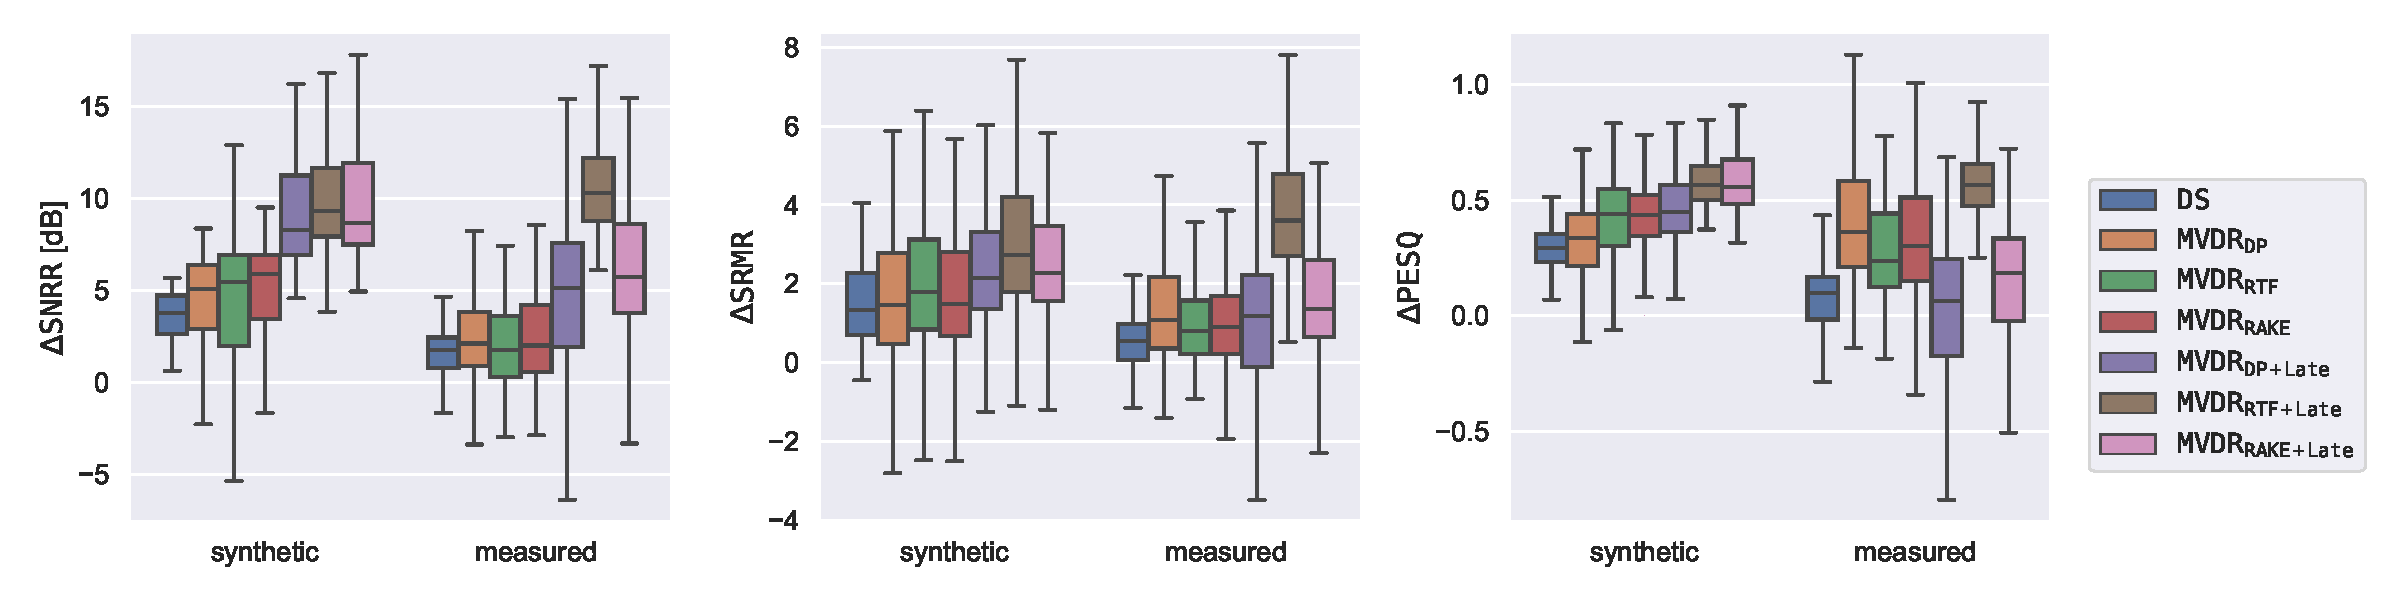
\includegraphics[trim={0 10 10 0},clip,width=\linewidth]{figures/dechorateapp/kowalkzy_results_boxplot.pdf}
        \caption{
        Comparison of echo-aware beamforming for the room configuration $\mathtt{011111}$ ($\RT \approx 600 $ ms) on measured and synthetic data  for all combinations of source-array positions in the \dEchorate{} dataset.}
        \label{fig:dechorateapp:se:results}
    \end{fullwidth}
\end{figure}

\newthought{Numerical results} are reported in Figure~\ref{fig:dechorateapp:se:results}.
When using synthetic data, the known echo timings perfectly match the components in the simulated \RIRs/, and, likewise, the echo model matches the \RIRs/' early part.
Here, one can see that more information is used, the better performances are. \ReTF/- and Rake- beamformers outperform the simple designs based on the direct path, and including the late reverberation statistics considerably boosts performance in all cases.
Interestingly, \ReTF/ have a slight edge over Rake-versions in terms of mean \ac{SNRR}.
This can be explained by the fact that \ac{GEVD} methods tend to robustly consider the stronger and more stable components of the \ReTFs/, which in reverberant and noisy static scenarios may identify with the earlier portion of the \RIRs/.
Moreover, since it is not constrained by a fix echo model, the \ReTFs/ can capture more information which, in turn, yields to sightly better enhancement.
Nevertheless, the \ac{PESQ} metrics suggest that for this ideal scenario  both echo-aware (Rake) and echo-agnostic (\ReTF/) design are comparable.
\\When it comes to measured \RIRs/, the trends are different.
Here, the errors in echo estimation, due to calibration mismatch and the richness of the acoustic propagation, lead to a drop in the performances for echo-aware methods, both in terms of means and variances.
This is even clearer when considering the $\dPESQ$ metric, as it also accounts for artifacts.
Here, the echo-agnostic beamformer considering late reverberation $\MVDR_\mathtt{ReTF+Late}$ outperforms the other methods, maintaining the trend exhibited on simulated data.
In general, it looks like the $\MVDR_\texttt{Rake+Late}$ has more variance than $\MVDR_\texttt{ReTF+Late}$, suggesting that in some situations, it performs better, while in other it performs less well.
This is probably due to the tiny annotation mismatch and the complexity of the \RIRs/ and future work will be devoted in a deeper in understanding of the underlying factors.
% Another promising research direction for echo-aware methods is to fine tune echo properties from data.

\section{Room Geometry Estimation}\label{sec:dechorateapp:rooge}
In this section, we shortly present another application of the \dEchorate{} dataset: \RooGEdef/, namely, the task of estimating the shape of a room knowing the positions of first-order image sources.
This problem is typically addressed by solving multiple instances of \textit{reflector localization}, aiming at estimating the position of a single surface (\eg/ wall, floor, \etc/).
\\Several methods have been proposed which take into account different levels of prior information and noise.
They were briefly discussed in the context of echo labeling in~\cref{subsec:estimation:active_rir}.
In general, these methods can be decomposed into three successive steps:
\begin{enumerate}
    \item echo labeling, in order to associate the echoes to image sources using one of the methods mentioned in~\cref{subsec:estimation:active_rir};
    \item estimation of the image source position either through  multilateration\citeonly{dokmanic2013acoustic, dokmanic2015relax}, \MLdef/\citeonly{tervo2011localization} or convex optimization~\citeonly{crocco2012closed};
    \item and finally, the \textit{image-source-reversion}, in order to localize the reflector, based on the geometrical assumption of the \ISMdef/.
\end{enumerate}
More advance techniques have been proposed in the literature of reflector localization for different setups and scenarios.
A comprehensive review can be found in \citeonly{remaggi2016acoustic, crocco2017uncalibrated}.
\\Nonetheless, when the echoes' \TOAs/ and their labeling are known for 4 spatially-separated non-coplanar microphones, one can perform this task using closed-form multilateration algorithms.

\subsection{Room Geometry Estimation through multilateration}
Multilateration is the problem of recovering the position of a point in the space from multiple distances between the point and known spatially-separated locations.
It is the 3D extension of the \textit{trilateration} problem, namely, determining an unknown position based on the distance to two other known vertices of a triangle.
In the context of \RooGE/, the distances from the source to the microphones can be obtained by converting the \TOAs/ [seconds] into distances [meters].
Then, the 3D coordinates of each image source can be retrieved, solving a convex problem as described in \citeonly{Beck2008ExactProblems}.
Ideally, this problem can be solved in closed-form.
However, due to measurement error (\eg/ errors in estimating the image's \TOAs/), it may be ill-conditioned.
To overcome this, the algorithm proposed in \citeonly{Beck2008ExactProblems} relies on a robust iterative approach yielding accurate solutions.
Finally, the position and orientation of each wall can be easily derived from the \ISM/ as the plane bisecting the line joining the real source position and the position of its corresponding image (see Figure~\ref{fig:dechorateapp:wall_rec}).

\begin{figure}[t]
    \begin{fullwidth}
    \centering
    \subfloat[image][Source images estimation]{
    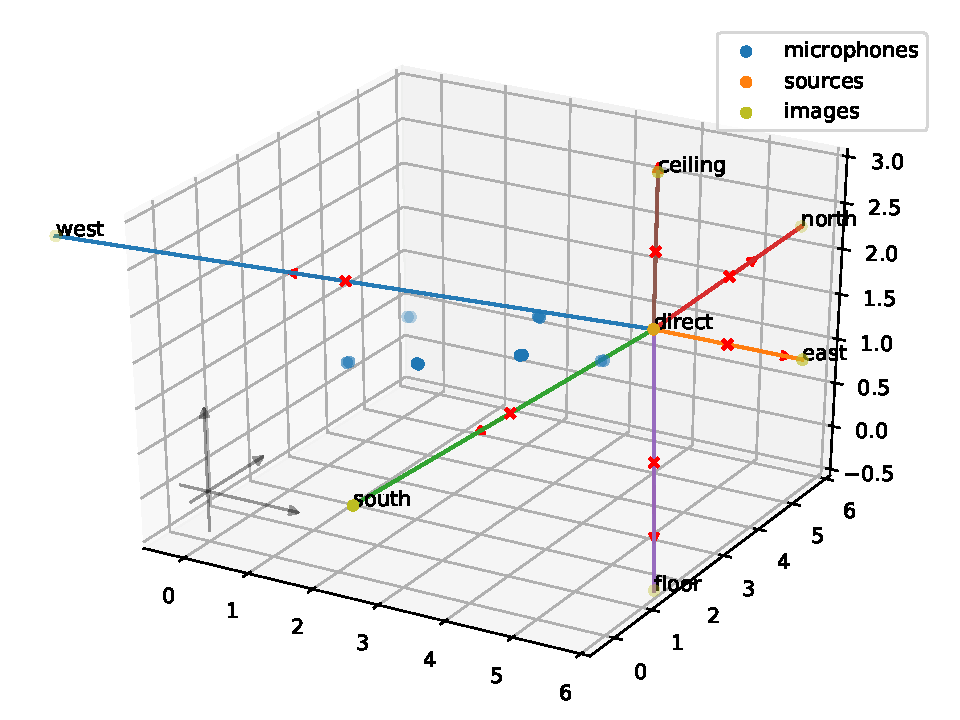
\includegraphics[width=0.48\textwidth]{figures/dechorate/estimated_image}
        \label{fig:dechorateapp:image}
    }
    \hfill
    \subfloat[reflector][Reflector estimation]{
        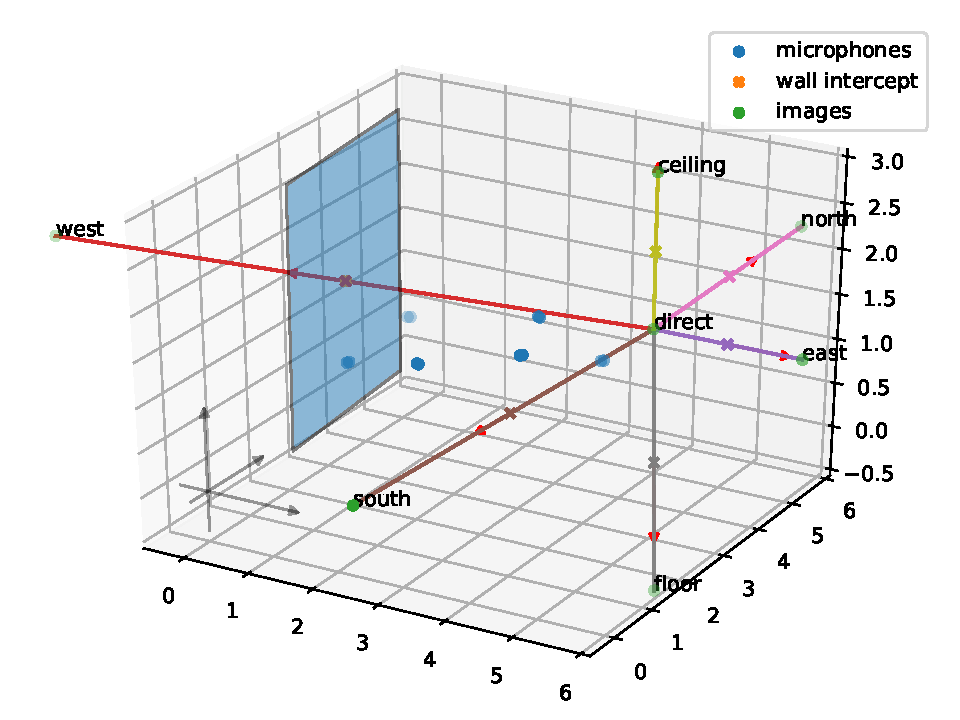
\includegraphics[width=0.48\textwidth]{figures/dechorate/estimated_reflector}
        \label{fig:dechorateapp:reflector}
    }
    \caption{Images source estimation (right) and corresponding reflector estimation (left) for one of the sound sources in the \acs{DECHORATE} dataset.}
    \label{fig:dechorateapp:wall_rec}
    \end{fullwidth}
\end{figure}

\subsection{Using the \dEchorate{} dataset for \acs{RooGE}}\label{subsec:dechorateapp:rooge}
In \dEchorate{}, the annotation of all the first-order images of sound sources is available.
We used the \citeauthor{Beck2008ExactProblems}'s multilateration method (available in the Python library \dEchorate{}) to estimate the image source position of each of the direct source using 6 non-coplanar microphones (on for each of the 6 arrays).
Then, room facets are estimated using each of the sources as a probe.
\cref{tab:res_rooge} shows the results of the estimation of the wall positions in terms of distance error (in centimeters) and surface orientation error (in degrees).
These metrics were previously used in the literature of reflector estimation, such as in~\citeonly{annibale2012geometric,crocco2017uncalibrated}.
\cref{fig:dechorateapp:reflector} depicts an example of reflector estimation using the \dEchorate{} data.

\begin{table}[h!]
    \begin{sidecaption}[]{
        Distance errors (DE) in centimeters and angular errors (AE) in degrees between ground truth and estimated room sides using each of the sound source (\#1 to \#4) as a probe.
        For each facet, bold font is used in correspondence to the source yielding the best DE and AE; while, italic font highlights outliers.
        }[tab:res_rooge]
    \centering
    \small
    \begin{tabular}{c|cc|cc|cc|cc}
\toprule
source id &	1	& &	2	& &	3	& &	4 &	\\
wall &	DE&	AE&	DE&	AE&	DE&	AE&	DE&	AE\\
\hline
west &	0.74	& $\ang{8.99}$      & 4.59	& $\ang{8.32}$  & 5.89	& $\ang{5.75}$	& $\mathbf{0.05}$    & $\mathbf{\ang{2.40}}$\\
east &	$\mathbf{0.81}$	& $\mathbf{\ang{0.08}}$      & 0.9	& $\ang{0.50}$	&$\mathit{69.51}$	& $\mathit{\ang{55.70}}$	& 0.31    & $\ang{0.21}$\\
south&	3.94	&$\ang{16.08}$      & $\mathbf{0.18}$	& $\ang{1.77}$	&$\mathit{14.37}$ & $\mathit{\ang{18.55}}$	& 0.82    & $\mathbf{\ang{1.65}}$\\
north&	1.34	& $\ang{0.76}$	    & 1.40	& $\ang{8.94}$	& $\mathbf{0.63}$	& $\mathbf{\ang{0.17}}$	& 2.08    & $\ang{1.38}$\\
floor&	$\mathbf{5.19}$	& $\mathbf{\ang{1.76}}$	    & 7.27	& $\ang{2.66}$	& 7.11	& $\ang{2.02}$	& 5.22    & $\ang{1.90}$\\
ceiling&1.16	& $\ang{0.28}$	    & 0.67	& $\ang{0.76}$	& $\mathbf{0.24}$	& $\ang{1.16}$	& $0.48$    & $\mathbf{\ang{0.26}}$\\

\bottomrule
\end{tabular}

    \end{sidecaption}
\end{table}

\mynewline
Despite a few outliers, the majority of the facets are estimated correctly in terms of their placement and orientation with respect to the coordinate system.
For instance, for source $\#4$, all 6 surfaces were localized within less than $6$~cm and $\ang{2.5}$ errors.
Small errors are due to concurrency of multiple factors, such as tiny offsets in the annotation and the ideal shoebox approximation\sidenote{
    In the real recording room, some gaps were present between revolving panels in the walls}.
It is also possible that for some source-receiver pairs, the far-field assumption is not verified, causing the inaccuracy of \textit{reverting} the \ISM/.
Finally, the 2 outliers for the source \#3 are due to a wrong annotation caused by the source directivity and misclassification.
In particular, when a wall is ``behind'' the source, the energy of the related reflection is very small and might not appear in the \RIRs/.
This happened for the eastern wall, and a second-order image was taken instead.
Secondly, the contribution of multiple reflections arriving at the same time can be merged into signal spikes in estimated \RIRs/.
This effect is particularly amplified when the microphones and loudspeakers exhibit long impulse responses.
As a consequence, some spikes were probably miss-classified.
This can be noticed for the southern-wall were again a second-order image was taken instead.
Nevertheless, this second type of error can be manually corrected, and the annotations updated.

\section{Conclusions}\label{sec:dechorateapp:conclusion}
In this chapter, we presented two applications of the \dEchorate{} dataset described in~\cref{ch:dechorate}: echo-aware spatial filtering and room geometry estimation.
\\The first one deals with the possibility of using early echoes to enhance a target speech signal corrupted by diffuse noise and a high level of reverberation.
To this end, two types of state-of-the-art spatial filtering criteria are considered: echo-agnostic and echo-aware beamformers.
Experimental results on real and synthetic data, both available in the proposed dataset, led to the following findings.
The synthetic data were computed using \ISM/-based simulation; thus, the early parts of \RIRs/ match the early echo model.
Therefore, replacing the acoustic vectors with few know echoes gives significant enhancement performance gains compared with baseline methods, which consider only the direct ideal propagation.
In this scenario, both echo-aware and state-of-the-art \ReTF/-based echo-agnostic perform similarly, suggesting the effectiveness of echo-aware approaches.
However, when using the corresponding real data available in the dataset, performances drop in terms of perceptual quality as predicted by the \acs{PESQ} score.
This may be due to the small mismatches between real and annotated echoes and the richness of the acoustic field, which impact the echo-aware methods.
The best-performing method is the echo-agnostic one based on \ReTF/, which does not suffer from any echo mismatch and can include other information about the acoustic propagation.
\\The relatively lower performance of rake-based filters on real scenarios than simulated ones emphasizes the importance of having precise enough \AER/ algorithms and encourages further studies on these echo-aware methods.
Moreover, the knowledge of the very same echoes is limited to spatial filtering and can be used to retrieve the entire room geometry, as demonstrated in the second section of this chapter.
\\By using standard approaches based on geometrical reasoning and robust multilateration algorithms, it is possible to revert the \ISM/ and map echoes' \TOAs/ to source and image-source position.
Here, we showed this on the \dEchorate data both as an application and as a way to validate the dataset.
Although the results highlight that some echo \TOAs/ have not been correctly classified, the overall annotation is consistent with the actual room planimetry.
Finally, we would like to mention that the best of our knowledge, this is the very first dataset of this kind, that is, featuring real data with full echo/image-source annotations.

\mynewline
\\Future works will explore several directions.
\begin{itemize}
    \item By making this dataset freely available to the audio signal processing community, we hope to foster research in AER and echo-aware to improve the performance of existing methods on real data.
    \item The dataset could be updated by including more robust annotations derived from more advanced algorithms for calibration and \AER/.
    \item regarding the applications, the echo-aware methods presented above could be validated over more challenging scenarios than the one presented.
    Such scenarios, \eg/ the presence of interfering sound sources and challenging levels of \SNR{} and \RT{}, are already included in the dataset, but not used in the evaluation above.
    \item By the amount of the data collected, they can be used to train learning-based signal processing methods or for data augmentation.
\end{itemize}
In a more long-term perspective, the data analysis conducted in this chapter brings the attention to exploring the impact of mismatch between simulated and real \RIR/ on audio signal processing methods.
Moreover, by using the pairs of simulated \vs/ real \RIRs/ available in the dataset, develop techniques to convert one to the other, using style transfer and domain adaptation techniques.
\qed
